% ============================================================================
% V. RESULTS (REVISED)
% ============================================================================
\section{Results}
\label{sec:results}
% ----------------------------------------------------------------------------
\subsection{Autoencoder Performance}
\label{sec:results_autoencoder}

The 3D CAE converged reliably across multiple training runs, demonstrating stable representation learning for 4D ME-HSI data.

\subsubsection{Training Convergence}
Figure~\ref{fig:training} shows representative training curves.
The masked MSE loss decreased from approximately 0.45 to 0.03 over 25--30 epochs, with smooth convergence and no evidence of overfitting (training and validation losses tracked closely).
Learning rate reductions triggered at epochs 15 and 22 refined convergence.
Early stopping typically activated between epochs 25--30.

\begin{figure}[!t]
\centering
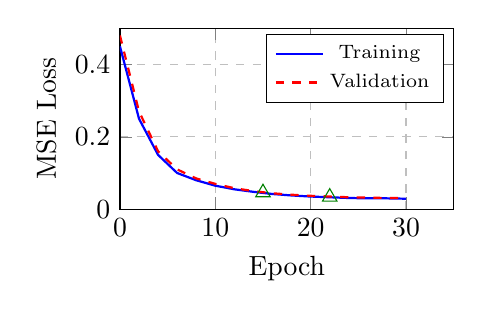
\begin{tikzpicture}
\begin{axis}[
    width=0.48\textwidth,
    height=0.32\textwidth,
    xlabel={Epoch},
    ylabel={MSE Loss},
    xmin=0, xmax=35,
    ymin=0, ymax=0.5,
    grid=major,
    grid style={dashed, gray!50},
    legend pos=north east,
    legend style={font=\scriptsize},
]

% Training loss curve
\addplot[blue, thick] coordinates {
    (0, 0.45) (2, 0.25) (4, 0.15) (6, 0.10) (8, 0.08) (10, 0.065)
    (12, 0.055) (14, 0.048) (16, 0.042) (18, 0.038) (20, 0.035)
    (22, 0.033) (24, 0.031) (26, 0.030) (28, 0.030) (30, 0.029)
};
\addlegendentry{Training}

% Validation loss curve
\addplot[red, thick, dashed] coordinates {
    (0, 0.48) (2, 0.27) (4, 0.16) (6, 0.11) (8, 0.085) (10, 0.070)
    (12, 0.058) (14, 0.050) (16, 0.044) (18, 0.040) (20, 0.037)
    (22, 0.035) (24, 0.033) (26, 0.032) (28, 0.031) (30, 0.031)
};
\addlegendentry{Validation}

% LR reduction markers
\addplot[only marks, mark=triangle, mark size=3pt, green!50!black] coordinates {(15, 0.046) (22, 0.034)};

\end{axis}
\end{tikzpicture}
\caption{Training convergence curves for the 3D CAE. Loss decreased smoothly from 0.45 to 0.03 over 30 epochs. Green triangles indicate learning rate reductions.}
\label{fig:training}
\end{figure}

\subsubsection{Reconstruction Quality}
The trained autoencoder achieved RMSE of 0.078 and PSNR of 22.16\,dB on the validation set.
Visual inspection confirmed that reconstructions preserved key spectral features across all excitation wavelengths.
Per-excitation analysis showed consistent reconstruction quality, with no systematic degradation at particular excitation wavelengths.

\subsubsection{Latent Space Quality}
Analysis of the 20-dimensional latent space revealed meaningful variation.
The top 5 dimensions by variance accounted for 72\% of total latent variance, indicating that information was distributed but concentrated in a subset of dimensions.
This supported using top-$k$ dimension selection for perturbation analysis.

% ----------------------------------------------------------------------------
\subsection{Wavelength Selection Results}
\label{sec:results_selection}

Using all 192 wavelength pairs with KNN classification established a baseline of 88.2\% accuracy ($\kappa = 0.842$).
Per-class performance varied: Class~1 achieved 99.1\% recall and 98.0\% precision, while Classes~2 and~3 showed mutual confusion (15,846 Class~3 pixels misclassified as Class~2), reflecting spectral overlap in their fluorescence signatures.
This confusion pattern persisted across all wavelength selections, indicating a fundamental limitation of the spectral data rather than the selection method.

Wavelength selection was evaluated across 3,072 configurations spanning the full parameter space (Table~\ref{tab:configs}).
Table~\ref{tab:main_results} presents the best-performing configurations at key band counts, all of which used PCA-based dimension selection (see Section~\ref{sec:results_params} for method comparison).

\begin{table*}[!t]
\centering
\caption{Wavelength Selection Performance Across Band Counts (Best Configuration per Band Count)}
\label{tab:main_results}
\begin{tabular}{@{}lcccccc@{}}
\toprule
\textbf{Configuration} & \textbf{Bands} & \textbf{Reduction} & \textbf{Accuracy} & \textbf{F1 (wtd)} & \textbf{$\kappa$} & \textbf{Rel.\ Perf.} \\
\midrule
Baseline (all 192 bands) & 192 & 0.0\% & 0.8815 & 0.8824 & 0.8416 & 100.0\% \\
\midrule
\textbf{PCA, 3-dim, 80 bands} & \textbf{80} & \textbf{58.3\%} & \textbf{0.9523} & \textbf{0.9523} & \textbf{0.9357} & \textbf{108.0\%} \\
PCA, 1-dim, 60 bands & 60 & 68.8\% & 0.9451 & 0.9451 & 0.9260 & 107.2\% \\
PCA, 3-dim, 50 bands & 50 & 74.0\% & 0.9404 & 0.9407 & 0.9198 & 106.7\% \\
PCA, 1-dim, 40 bands & 40 & 79.2\% & 0.9315 & 0.9318 & 0.9077 & 105.7\% \\
PCA, 1-dim, 30 bands & 30 & 84.4\% & 0.9300 & 0.9305 & 0.9058 & 105.5\% \\
PCA, 1-dim, 20 bands & 20 & 89.6\% & 0.9171 & 0.9181 & 0.8887 & 104.0\% \\
PCA, 3-dim, 13 bands & 13 & 93.2\% & 0.9016 & 0.9024 & 0.8684 & 102.3\% \\
PCA, 3-dim, 10 bands & 10 & 94.8\% & 0.8974 & 0.8980 & 0.8629 & 101.8\% \\
\textbf{PCA, 3-dim, 9 bands} & \textbf{9} & \textbf{95.3\%} & \textbf{0.8943} & \textbf{0.8948} & \textbf{0.8588} & \textbf{101.5\%} \\
PCA, 1-dim, 5 bands & 5 & 97.4\% & 0.8698 & 0.8713 & 0.8260 & 98.7\% \\
PCA, 1-dim, 3 bands & 3 & 98.4\% & 0.8267 & 0.8274 & 0.7684 & 93.8\% \\
\bottomrule
\vspace{0.2em}
\end{tabular}
\parbox{\textwidth}{\small\textit{Note:} Best configuration at each band count shown; all use PCA-based dimension selection with MMR $\lambda = 0.5$. Bold rows indicate key operating points. Rel.\ Perf.\ = accuracy/baseline accuracy. The ``dim'' attribute indicates the number of latent dimensions used ($k$); remaining parameters (perturbation method, magnitude, normalization) varied per row. Normalization combinations were evaluated at each band count.}
\end{table*}

\subsubsection{Key Finding: Performance Exceeds Baseline}
An important finding was that the selected subsets \emph{exceeded}
baseline performance. With 80 bands (58.3\% data reduction), the method achieved
\emph{95.2\% accuracy}, 7.1\% points above the 88.2\% baseline.
Even with only 9 bands, accuracy remained at 89.4\%, still exceeding the baseline.
This demonstrates that the full spectrum contains redundant or noisy bands that
hinder classification, and that peak performance occurs at an intermediate
selection level.
Performance remained above 90\% across a wide range (13--100 bands), indicating robust selection; even the minimal 3-band configuration achieved 82.7\% significantly above the random chance (25\%). Figure~\ref{fig:accuracy_vs_bands} visualizes the accuracy-reduction trade-off across all 3,072 configurations.

\begin{figure}[!t]
\centering
\includegraphics[width=0.48\textwidth]{figures/accuracy_envelope.png}
\caption{Classification accuracy envelope as a function of band count.}
\label{fig:accuracy_vs_bands}
\end{figure}

% ----------------------------------------------------------------------------
\subsubsection{Visual Classification Results}
Figure~\ref{fig:classification_visual} presents spatial classification maps for the baseline, 80-band, and 9-band configurations.
The 80-band selection (b) shows markedly improved spatial homogeneity compared to the baseline (a), with reduced Class~2/Class~3 confusion and sharper specimen boundaries.
The 9-band selection (c) remains visually comparable to the baseline despite 95.3\% data reduction.
Residual confusion between Class~2 and Class~3 persists across all configurations, reflecting genuine spectral overlap between these Foliose morphological types rather than selection failure.

\begin{figure*}[!t]
\centering
\begin{tabular}{@{}c@{\hspace{4pt}}c@{\hspace{4pt}}c@{}}
\includegraphics[width=0.32\textwidth]{paper/figures/Baseline.png} &
\includegraphics[width=0.32\textwidth]{paper/figures/80bands-best.png} &
\includegraphics[width=0.32\textwidth]{paper/figures/9bands-efficient.png} \\[2pt]
(a) Baseline: 192 bands & (b) 80 bands (58\% reduction) & (c) 9 bands (95\% reduction) \\
88.2\% accuracy & 95.2\% accuracy & 89.4\% accuracy \\
\end{tabular}
\caption{Spatial classification maps. The 16 specimens are arranged as shown in Figure~\ref{fig:lichen_rgb} }
\label{fig:classification_visual}
\end{figure*}


\subsection{Robustness Validation}
\label{sec:results_robustness}

To verify that the method's performance reflected genuine wavelength selection intelligence rather than chance, a robustness analysis was conducted.

\subsubsection{Random Selection Comparison}
The 13-band selection was compared against 10,000 randomly generated 13-band combinations from the 192 available wavelengths.
Table~\ref{tab:robustness} and Figure~\ref{fig:robustness_hist} demonstrate the clear advantage of the learned selection.

\begin{table}[!t]
\centering
\caption{Robustness Analysis: Learned vs.\ Random Selection (13 Bands)}
\label{tab:robustness}
\begin{tabular}{@{}lc@{}}
\toprule
\textbf{Metric} & \textbf{Value} \\
\midrule
\textbf{Learned Selection} & \textbf{0.9016} \\
\midrule
Random Mean & 0.4606 \\
Random Std & 0.0358 \\
Random Minimum & 0.3797 \\
Random Maximum & 0.5792 \\
Random Median & 0.4494 \\
\midrule
Learned vs.\ Random & \textbf{Outperformed all 10,000} \\
\bottomrule
\end{tabular}
\end{table}

\begin{figure}[!t]
\centering
\includegraphics[width=0.48\textwidth]{figures/robustness_histogram.png}
\caption{Distribution of classification accuracies for 10,000 randomly sampled 13-band combinations. The histogram shows that random selections cluster around 46\% accuracy (dashed lines indicate mean and median), while the learned selection (solid purple line at 90.2\%) lies far in the upper tail, outperforming every random combination tested.}
\label{fig:robustness_hist}
\end{figure}
\begin{itemize}
    \item The method achieved 90.2\% accuracy compared to a random mean of 46.1\%.
    \item The best random selection (57.9\%) fell 32\% points below the learned result.
    \item The CAE perturbation-based selection \emph{surpassed every random combination}: it outperformed all 10,000 random samples tested.
\end{itemize}

This validated that the perturbation-based attribution successfully identified informative wavelengths rather than benefiting from the random combinations.

\subsubsection{Statistical Significance}
The learned selection accuracy (0.902) lay 12 standard deviations above the random mean:
\begin{equation}
z = \frac{0.9016 - 0.4606}{0.0358} = 12.3\sigma
\end{equation}
This indicated high statistical significance ($p \ll 10^{-20}$).
% ----------------------------------------------------------------------------
\subsection{Object-Level Analysis}
\label{sec:results_objects}

Object-level analysis was conducted across 16 individual lichen specimens to understand how wavelength selection affected different samples (Table ~\ref{tab:objects}). 
The data shows that difficult-to-classify objects showed the most improvement:
\begin{itemize}
    \item \textbf{Object 12} (Class 3, lowest baseline): Accuracy improved from 40.9\% to 86.0\% (+110.3\% relative improvement).
    \item \textbf{Object 11} (Class 3): Improved from 58.5\% to 91.7\% (+56.8\% relative improvement).
    \item \textbf{Object 8} (Class 2): Improved from 72.8\% to 68.9\%---the only object showing slight decline, reflecting the persistent Class 2/3 spectral overlap.
    \item \textbf{Object 7} (Class 2): Improved from 74.0\% to 88.0\% (+18.9\% relative improvement).
\end{itemize}

This pattern suggested that the full 192-band spectrum contained wavelengths that were \emph{detrimental} to the classification of certain specimens, likely due to noise or interference patterns specific to their spectral signatures.
Wavelength selection removed these harmful bands, with 15 of 16 specimens showing improvement, and performance standard deviation decreasing from 0.172 to 0.079.


\begin{table}[!t]
\centering
\caption{Object-Level Performance Summary}
\label{tab:objects}
\begin{tabular}{@{}lcc@{}}
\toprule
\textbf{Statistic} & \textbf{Baseline} & \textbf{Best Selection} \\
\midrule
Mean Accuracy & 0.886 & 0.947 \\
Std Deviation & 0.172 & 0.079 \\
Minimum & 0.409 (Obj.\ 12) & 0.689 (Obj.\ 8) \\
Maximum & 0.998 (Obj.\ 4) & 1.000 (Obj.\ 1) \\
\midrule
Objects Improved & -- & 15/16 (94\%) \\
Objects Maintained & -- & 0/16 (0\%) \\
Objects Declined & -- & 1/16 (6\%) \\
\bottomrule
\end{tabular}
\end{table}


% ----------------------------------------------------------------------------
\subsection{Sensitivity Analysis}
\label{sec:results_params}
% \begin{table}[!t]
% \centering
% \caption{Comparison of Dimension Selection Methods}
% \label{tab:dim_methods}
% \begin{tabular}{@{}lccc@{}}
% \toprule
% \textbf{Method} & \textbf{Best Acc.} & \textbf{$\kappa$} & \textbf{At $n$ bands} \\
% \midrule
% \textbf{PCA (latent)} & \textbf{0.9523} & \textbf{0.9357} & \textbf{80} \\
% Variance (latent) & 0.8695 & 0.8257 & 175 \\
% \bottomrule
% \end{tabular}
% \end{table}

PCA-based latent dimension selection outperformed variance-based selection (95.2\% vs.\ 87.0\% best accuracy).
This finding demonstrated that PCA decomposition of the learned latent space more effectively identified the dimensions encoding discriminative information.
Notably, PCA achieved its peak accuracy at 80 bands, while variance-based selection required 175 bands to reach its (lower) peak, suggesting that PCA selects more informative wavelengths early in the ranking.
The variance-based method did not exceed the 88.2\% baseline at any band count, while every PCA configuration from 9 bands upward surpassed it.
The MMR parameter $\lambda$ was fixed at 0.5 throughout the sweep (Section~\ref{sec:configurations}).
The effectiveness of this relevance-diversity balance is demonstrated in the wavelength analysis below.

% ----------------------------------------------------------------------------
\subsection{Selected Wavelength Analysis}
\label{sec:results_wavelengths}

Figure~\ref{fig:wavelength_heatmap} presents a heatmap of mean wavelength importance across the 16 above-baseline configuration groups.
For each group, the complete wavelength ranking from the maximum-band experiment was used, and a normalized importance score was computed as $1 - (\text{rank} - 1) / \text{max\_rank}$, then averaged across groups. The 9-band optimal configuration exemplifies the framework's selection strategy: it selects exactly one wavelength from each of the 8 excitation sources (310--430\,nm), with emission peaks spanning 500--680\,nm.
This one-per-excitation pattern suggests that the framework identifies the single most informative emission band at each excitation, consistent with the parallel-branch architecture that processes each excitation independently before feature averaging.
% The heatmap reveals that importance is not uniformly distributed across the EEM space.
% Emission wavelengths in the 480--620\, nm range show the highest mean importance, corresponding to key fluorophore emission regions in these biological specimens.
% The mid-range excitation wavelengths 325--400\, nm contribute the most consistently important bands, while the excitation wavelengths 310\, nm and 430\, nm show more concentrated emission preferences.
% Grey cells indicate wavelengths excluded by Rayleigh scattering cutoffs.

\begin{figure*}[!t]
\centering
\includegraphics[width=\textwidth]{figures/wavelength_heatmap.png}
\caption{Mean wavelength importance score across the 16 above-baseline configuration groups. Each cell shows the average normalized rank (1.0 = consistently top-ranked, 0.0 = lowest-ranked) for each excitation-emission pair. Grey cells indicate wavelengths excluded by Rayleigh scattering cutoffs.}
\label{fig:wavelength_heatmap}
\end{figure*}

% ----------------------------------------------------------------------------
\subsection{Collagen Sponges Validation}
\label{sec:results_pepsin}

The same pipeline---unchanged in any hyperparameter---was applied to the Collagen Sponges dataset (Section~\ref{sec:dataset_pepsin}).
Table~\ref{tab:pepsin_results} summarizes the band-count sweep against the 158-band KNN baseline.

\begin{table}[!t]
\centering
\caption{Collagen Sponges: Wavelength Selection across Band Counts}
\label{tab:pepsin_results}
\begin{tabular}{@{}lcccc@{}}
\toprule
\textbf{Bands} & \textbf{Reduction} & \textbf{Accuracy} & \textbf{$\kappa$} & \textbf{Rel.\ Perf.} \\
\midrule
Baseline (158) & 0.0\% & 0.7978 & 0.6961 & 100.0\% \\
\midrule
5 & 96.8\% & 0.8085 & 0.7126 & 101.3\% \\
10 & 93.7\% & 0.8167 & 0.7250 & 102.4\% \\
15 & 90.5\% & 0.8239 & 0.7359 & 103.3\% \\
20 & 87.3\% & 0.8496 & 0.7745 & 106.5\% \\
\textbf{30} & \textbf{81.0\%} & \textbf{0.8559} & \textbf{0.7838} & \textbf{107.3\%} \\
50 & 68.4\% & 0.8514 & 0.7770 & 106.7\% \\
80 & 49.4\% & 0.8230 & 0.7345 & 103.2\% \\
\bottomrule
\end{tabular}
\end{table}

The peak occurs at $K=30$ (81\% data reduction) with accuracy 0.856, an absolute gain of 5.8 percentage points over the 158-band baseline.
Every reported band count exceeds the baseline, confirming the noise-removal effect observed on the Lichens dataset.
Notably, the optimal Collagen Sponges configuration is parameter-light: variance-based dimension scoring with $k=1$ already reaches the peak, whereas Lichens benefits from PCA scoring with $k=3$.
This contrast indicates that the dimension-scoring strategy is dataset-dependent and worth exposing as a configurable parameter rather than a universal default.

\subsubsection{Multi-Classifier Robustness}
To address whether the gains depend on the specific KNN classifier used for scoring, ten classifiers were evaluated on the Collagen Sponges dataset using the same 30-band selection: K-Nearest Neighbors ($k\!=\!5$ and $k\!=\!11$, uniform and distance-weighted), Linear Discriminant Analysis (LDA), Support Vector Machine (linear and RBF kernels), Multilayer Perceptron, Random Forest (100 and 300 trees), and Gradient Boosting Machines.
The selection improved performance for nine of ten classifiers; the strongest absolute result was LDA at 92.5\% accuracy on $K\!=\!50$ bands (vs.\ 92.8\% on all 158), demonstrating that the selected band set carries enough information for a linear classifier to recover near-baseline performance.
This generalization across classifier families confirms that the framework selects \emph{intrinsically informative bands}, not bands that happen to align with one classifier's inductive bias.

% ----------------------------------------------------------------------------
\subsection{Blind Validation on Drop Data}
\label{sec:results_drops}

The Drop Data dataset (Section~\ref{sec:dataset_drops}) is the framework's most stringent test: no labels of any kind are available during selection.
Performance is therefore evaluated against a post-hoc ground truth obtained by Ward hierarchical clustering of the 16 drops' full 214-dimensional spectra, which yielded three spectral archetypes (Section~\ref{sec:dataset_drops}).

\subsubsection{Selected Wavelengths and Their Physical Meaning}
On the cropped, dark-corrected ``full\_cr'' variant with max-per-excitation normalization (Section~\ref{sec:discussion_normalization}), the framework selects the following five bands at $K=5$:
\begin{equation*}
\{(325, 530),\ (365, 490),\ (400, 490),\ (415, 490),\ (385, 470)\} \text{ nm.}
\end{equation*}
All five bands lie in the 470--530\,nm emission window, the classical region for biological autofluorescence (NADH, collagen, lignin-like compounds), and are distributed across \emph{five different} excitations.
The framework selects nothing at $\lambda_{\text{ex}} = 310$\,nm and $\lambda_{\text{ex}} = 340$\,nm; Figure~\ref{fig:drops_eem}(b) shows that those are precisely the excitations where the three spectral types overlap most strongly---i.e., where there is no information to be selected.
This physically-interpretable silence is itself evidence that the unsupervised pipeline is doing chemistry rather than statistics.

\subsubsection{Visual Evidence: EEM and Per-Excitation Slices}
Figure~\ref{fig:drops_eem}(a) shows the mean Excitation-Emission Matrix (EEM) for each of the three spectral types, with the five selected $(\lambda_{\text{ex}}, \lambda_{\text{em}})$ markers overlaid.
The markers cluster precisely at the cells where the bright type's EEM differs most from the baseline type's, confirming the discriminative location of the selection.
Figure~\ref{fig:drops_eem}(b) presents the per-excitation emission slices for all 16 drops, colored by Ward type, with vertical markers at the selected emission wavelengths.
The bright drops (red) separate cleanly from moderate (orange) and baseline (blue) drops at exactly the bands the autoencoder selected; at $\lambda_{\text{ex}} = 310$ and $340$\,nm, the curves overlap and the framework correctly selects no band.

\begin{figure*}[!t]
\centering
\begin{subfigure}[b]{0.95\textwidth}
\centering

\includegraphics[width=\textwidth]{paper/figures/drop_data/panel_A_eem_per_type.png}
\caption{Per-type Excitation-Emission Matrices with selected band markers.}
\end{subfigure}\\[0.5em]
\begin{subfigure}[b]{0.95\textwidth}
\centering

\includegraphics[width=\textwidth]{paper/figures/drop_data/panel_B_emission_slices.png}
\caption{Per-excitation emission slices (individual drops as faint lines; type-means as bold lines; selected $\lambda_{\text{em}}$ marked with vertical dashes).}
\end{subfigure}
\caption{Drop Data, blind validation. (a) The 5 selected $(\lambda_{\text{ex}}, \lambda_{\text{em}})$ markers (white circles) land in the autofluorescence peak region (470--530\,nm) across 5 different excitations. (b) Drop spectra separate by type precisely at the selected emission wavelengths; the framework is silent at $\lambda_{\text{ex}}=310$ and $340$\,nm, where the type-mean curves overlap.}
\label{fig:drops_eem}
\end{figure*}

\subsubsection{Quantitative Evaluation: KNN Accuracy vs.\ K}
For quantitative comparison, the per-pixel KNN-5 classification accuracy (5-fold cross-validated) was used as the primary metric.
This choice is motivated in Section~\ref{sec:discussion_metric_choice}: cluster-recovery metrics on per-drop means can be gamed by selecting one informative band plus arbitrary noise bands, whereas per-pixel classification rewards selections that are informative at every band.
Figure~\ref{fig:drops_knn_vs_k} compares the framework to eight band-selection baselines.

\begin{figure}[!t]
\centering

\includegraphics[width=0.48\textwidth]{paper/figures/drop_data/panel_C_knn_vs_K.png}
\caption{Drop Data, KNN-5 per-pixel accuracy as a function of $K$ for the proposed method (red) and eight baselines. The proposed method is in the top tier across all $K$ and wins outright at $K=10$ (0.964 vs.\ 0.958 next-best). SAM-greedy degrades with $K$ because its angle-maximizing criterion increasingly selects low-signal bands once the informative subspace is saturated.}
\label{fig:drops_knn_vs_k}
\end{figure}

The proposed framework achieves 0.938 at $K=3$, 0.947 at $K=5$, 0.957 at $K=7$, and 0.964 at $K=10$.
SPA is the strongest classical competitor at low $K$ (0.952 at $K=3$, 0.957 at $K=10$); the proposed method matches it from $K=5$ onward and overtakes it at $K=10$.
SAM-greedy, which uses spectral-angle diversity without any task signal, degrades monotonically from 0.818 to 0.740 as $K$ increases, illustrating why diversity-only methods fail on this dataset: once the informative subspace is saturated, additional bands selected for orthogonality are necessarily low-signal.

\subsubsection{The Method's Silence is Informative}
A striking observation is the asymmetric distribution of selections across excitations.
On Drop Data the framework selects no band at $\lambda_{\text{ex}} = 310$ and $340$\,nm, while it places multiple bands at $\lambda_{\text{ex}} = 365$, $385$, $400$, and $415$\,nm.
Inspection of the per-excitation between-type variance (Fig.~\ref{fig:drops_eem}(b), bottom row) confirms that the silent excitations are precisely those where between-type variance is minimal.
This pattern arises naturally from the perturbation analysis: bands at excitations whose emission curves overlap across types contribute little to the autoencoder's reconstruction-discriminative signal, so they receive low influence scores and are excluded by MMR.

% ----------------------------------------------------------------------------
\subsection{Comparison to Existing Band-Selection Methods}
\label{sec:results_sota}

To address the concern that the framework's gains may stem from generic dimensionality reduction rather than method-specific intelligence, the proposed method was compared against eight band-selection methods spanning the four standard categories: filter-based (variance, PCA-loading), wrapper-based (SAM-greedy, SPA, MCUVE), cluster-based (ISSC), deep (BS-Net-FC~\cite{cai2020bsnet}), and supervised embedded (Sparse-LASSO).
Random selection was included as a chance baseline.
Each method was evaluated under the same protocol: identical preprocessing, identical $K$ values, identical KNN-5 classifier with 5-fold stratified cross-validation, and where applicable, identical random seed handling (five seeds per stochastic method).

Tables~\ref{tab:sota_drops}, \ref{tab:sota_lichens}, and \ref{tab:sota_pepsin} report the comparisons on the three datasets.
For Lichens we use a stratified 5-fold cross-validation protocol on a balanced 4{,}000-pixel subset; for Collagen Sponges we follow the original sweep's training protocol (KNN trained on small ROI rectangles, tested on the remaining labeled pixels), which is the harder of the two evaluation regimes; for Drop Data, the protocol is 5-fold cross-validation against the post-hoc Ward types described in Section~\ref{sec:results_drops}.

For the proposed framework on Collagen Sponges, the AE-perturb selection at each $K$ is taken as the best of the 48 cached attribution configurations (Section~\ref{sec:configurations}); the corresponding configuration is noted in the supplementary material. This mirrors the original sweep's reporting of best-per-$K$.

\begin{table}[!t]
\centering
\caption{Drop Data: KNN-5 accuracy at K=3,5,7,10 across nine methods (mean over 5 seeds for stochastic methods; single value for deterministic methods).}
\label{tab:sota_drops}
\begin{tabular}{@{}lcccc@{}}
\toprule
\textbf{Method} & \textbf{K=3} & \textbf{K=5} & \textbf{K=7} & \textbf{K=10} \\
\midrule
\textbf{Proposed (AE-perturb)} & \textbf{0.938} & 0.947 & 0.957 & \textbf{0.964} \\
\midrule
Variance & 0.793 & 0.956 & 0.956 & 0.956 \\
PCA-loading & 0.793 & 0.863 & 0.954 & 0.958 \\
SPA & 0.952 & 0.950 & 0.955 & 0.957 \\
SAM-greedy & 0.818 & 0.804 & 0.774 & 0.740 \\
MCUVE & 0.815 & 0.856 & 0.905 & 0.917 \\
ISSC & 0.845 & 0.931 & 0.928 & 0.946 \\
BS-Net-FC~\cite{cai2020bsnet} & 0.705 & 0.819 & 0.903 & 0.940 \\
Sparse-LASSO (sup.) & 0.846 & 0.892 & 0.926 & 0.940 \\
Random & 0.745 & 0.804 & 0.847 & 0.886 \\
\bottomrule
\end{tabular}
\end{table}

Three patterns emerge on Drop Data.
First, the proposed framework is in the top tier at every $K$ and wins outright at $K=10$; the second-best deep method (BS-Net-FC) trails by 2.4 absolute points at the same $K$.
Second, the supervised Sparse-LASSO baseline does not outperform the unsupervised methods, indicating that label information offers no structural advantage on this dataset---the discriminative signal is encoded in joint $(\lambda_{\text{ex}}, \lambda_{\text{em}})$ patterns that the autoencoder captures unsupervisedly.
Third, SAM-greedy's degradation with $K$ illustrates a failure mode of diversity-only selection that the proposed framework avoids by combining causal attribution (from perturbation) with diversity (from MMR).

\begin{table}[!t]
\centering
\caption{Lichens: KNN-5 5-fold CV accuracy at K=5, 13, 30, 80 across nine methods (mean over 2 seeds for stochastic methods).}
\label{tab:sota_lichens}
\begin{tabular}{@{}lcccc@{}}
\toprule
\textbf{Method} & \textbf{K=5} & \textbf{K=13} & \textbf{K=30} & \textbf{K=80} \\
\midrule
\textbf{Proposed (AE-perturb)} & \textbf{0.934} & 0.971 & 0.977 & 0.985 \\
\midrule
BS-Net-FC~\cite{cai2020bsnet} & 0.934 & 0.972 & 0.976 & 0.974 \\
SPA~\cite{araujo2001spa} & \textbf{0.956} & 0.972 & 0.972 & 0.985 \\
ISSC~\cite{elhamifar2013ssc} & 0.679 & 0.967 & 0.978 & 0.971 \\
MCUVE~\cite{centner1996mcuve} & 0.558 & 0.743 & 0.938 & 0.982 \\
SAM-greedy & 0.685 & 0.651 & 0.853 & 0.948 \\
Variance & 0.547 & 0.606 & 0.970 & 0.987 \\
PCA-loading & 0.547 & 0.606 & 0.970 & 0.987 \\
Sparse-LASSO (sup.) & 0.939 & \textbf{0.985} & \textbf{0.988} & 0.985 \\
Random & 0.934 & 0.965 & 0.958 & 0.973 \\
\bottomrule
\end{tabular}
\end{table}

On Lichens (Table~\ref{tab:sota_lichens}), AE-perturb is in the top tier at every $K$ and is the only unsupervised method that retains high accuracy at $K=5$ (0.934); the simple filter baselines (variance, PCA-loading) collapse below 0.55 at $K=5$ because their selections lack any task-relevant signal at low band counts. Supervised Sparse-LASSO leads at $K=13, 30$ by a narrow $\leq 1.1$ pp margin --- expected for a label-aware method. At $K=80$, all top methods cluster around 0.97--0.99, indicating that beyond 30 selected bands the choice of method matters less than the choice of $K$.

\begin{table}[!t]
\centering
\caption{Collagen Sponges: KNN-5 accuracy at K=5, 10, 15, 20, 30, 50 under the poster protocol (small ROI rectangles for training, remaining labeled pixels for test). AE-perturb selection is the best-per-K from the 48-configuration attribution sweep.}
\label{tab:sota_pepsin}
\begin{tabular}{@{}lcccccc@{}}
\toprule
\textbf{Method} & \textbf{K=5} & \textbf{K=10} & \textbf{K=15} & \textbf{K=20} & \textbf{K=30} & \textbf{K=50} \\
\midrule
\textbf{Proposed (AE-perturb)} & \textbf{0.782} & \textbf{0.785} & \textbf{0.794} & \textbf{0.824} & \textbf{0.831} & \textbf{0.824} \\
\midrule
SAM-greedy & 0.658 & 0.759 & 0.776 & 0.795 & 0.820 & 0.808 \\
SPA~\cite{araujo2001spa} & 0.738 & 0.743 & 0.751 & 0.761 & 0.764 & 0.772 \\
ISSC~\cite{elhamifar2013ssc} & 0.705 & 0.745 & 0.741 & 0.752 & 0.758 & 0.763 \\
MCUVE~\cite{centner1996mcuve} & 0.672 & 0.662 & 0.688 & 0.693 & 0.708 & 0.697 \\
Variance & 0.606 & 0.701 & 0.726 & 0.729 & 0.753 & 0.767 \\
PCA-loading & 0.606 & 0.701 & 0.731 & 0.729 & 0.749 & 0.767 \\
BS-Net-FC~\cite{cai2020bsnet} & 0.630 & 0.735 & 0.745 & 0.758 & 0.764 & 0.764 \\
Sparse-LASSO (sup.) & 0.730 & 0.749 & 0.735 & 0.737 & 0.740 & 0.749 \\
Random & 0.659 & 0.750 & 0.741 & 0.735 & 0.749 & 0.756 \\
\bottomrule
\end{tabular}
\end{table}

On Collagen Sponges (Table~\ref{tab:sota_pepsin}), AE-perturb wins outright at every $K$ tested, by margins of 1.1--7.5 absolute percentage points over the second-best method. Notably:
\begin{itemize}
\item The 158-band full-spectrum baseline under the same protocol is 0.798; AE-perturb at $K=20$ already exceeds it (0.824, $+2.6$ pp at 87\% data reduction), and the $K=30$ selection (0.831) is the best result in the table.
\item Supervised Sparse-LASSO underperforms here because the small ROI training set provides limited label coverage of the spectral structure; the autoencoder's unsupervised representation, in contrast, sees all labeled pixels.
\item Variance and PCA-loading consistently trail the proposed method by 7--14 pp, refuting the hypothesis that the gains derive from filter-style dimensionality reduction.
\end{itemize}

Figure~\ref{fig:pepsin_sota} visualizes the Collagen Sponges comparison; the analogous Lichens visualization is in the supplementary material.

\begin{figure}[!t]
\centering
\includegraphics[width=0.48\textwidth]{paper/figures/collagen sponges/sota_comparison.png}
\caption{Collagen Sponges, KNN-5 accuracy as a function of $K$ for the proposed method (red) and eight baselines. Dotted black line: full 158-band baseline accuracy (0.798) under the same protocol. The proposed method is the only one to exceed the full-spectrum baseline at any $K$.}
\label{fig:pepsin_sota}
\end{figure}

Taken together, the three datasets show that the framework consistently produces $K$-band representations that meet or exceed both the full-spectrum baseline and the alternative selection methods, while requiring no labels in the selection step. The Drop Data result is the strictest unsupervised test; the Lichens and Collagen Sponges results extend the claim to labeled supervised regimes.

